\documentclass{article}

\usepackage{listings}
\usepackage{graphicx}
\usepackage{cite}
\usepackage{url}
\usepackage{listings}
\usepackage[margin=0.75in]{geometry}
\usepackage{color}

\title{LIGO Compatible Beam-Splitter Optical Fiber Construction Procedure}
\author{M.P.Ross}
\begin{document}
\maketitle
\section{Introduction}
This document describes the procedure to create a beam splitter optical fiber that satisfies the LIGO vacuum compatibility requirements [1]. The final product is a optical fiber with a flat faced beam-splitter tip on one end and an angled connector on the other that can then be used for cBRS fiber interferometer readouts. The use of a flat faced connector is necessary to allow the reflected beam to couple back through the fiber while the angled connection is utilized to decrease spurious reflection when connected to other optical fiber components.
\section{Materials}
\begin{itemize}
\item 1 (+extras) FC/APC optical fiber connector
\item 1 (+extras) FC/PC optical fiber connector
\item Nufern S1310-P (Polymide coated fiber)
\item Epo-Tek 353ND (UHV epoxy)
\end{itemize}
\section{Steps}
\begin{enumerate}
\item Clean connectors in an ultrasonic cleaner of deionized water or alcohol for roughly ten minutes. Make sure to clean more connectors than you need as they will become unusable if the fiber breaks while threading. 
\item Strip an inch long section of the fiber using a household lighter. Gently "brush" the flame over the fiber many times until the polymide is completely burnt away then clean the section with an alcohol soaked Kim-wipe and finally blow off with compressed air.
\item Connectorize the fiber with a FC/APC connector on one end and a FC/PC connector on the other by following the Thorlabs Guide to Connectorization and Polishing Optical Fibers while omitting all steps pertaining to non-vacuum compatible pieces. Specifically do not include the strain relief or the jacket material. Additionally, use Epo-Tek 353ND instead of the given epoxy. Be especially gentle while threading the fiber through the ferule as it will be brittle due to the polymide removal. If fiber gets stuck while threading, remove, clean both the fiber and ferule, and reflame fiber tip before trying again.
\item Insert into sputterer and connect angle end to feed through and flat end to a mount over the sputtering source.
\item Connect cBRS readout box to the feed through using a patch cable.
\item Cover fiber except for the very tip to keep gold off the rest of the fiber.
\item Ensure that light is being emitted out of the tip.
\item Close up and sputter following the below guide.
\end{enumerate}
\section{Gold Sputterering}
During this procedure the gold sputterering is monitored in situ using the cBRS readout optics and electronics. The optical set up is a 1310 nm fiber coupled laser which passes through a circulator and out to the chamber. The other connection of the circulator connects to a Thorlabs photodiode to monitor the return beam. This set up allows the measurement of the reflectance of the fiber in real time.\\

\textbf{Settings:}

Mass Controler: 31

Argon Pressure: 7.2 mTorr

Gold Power: 15 W

Rate: 0.3 \AA/sec

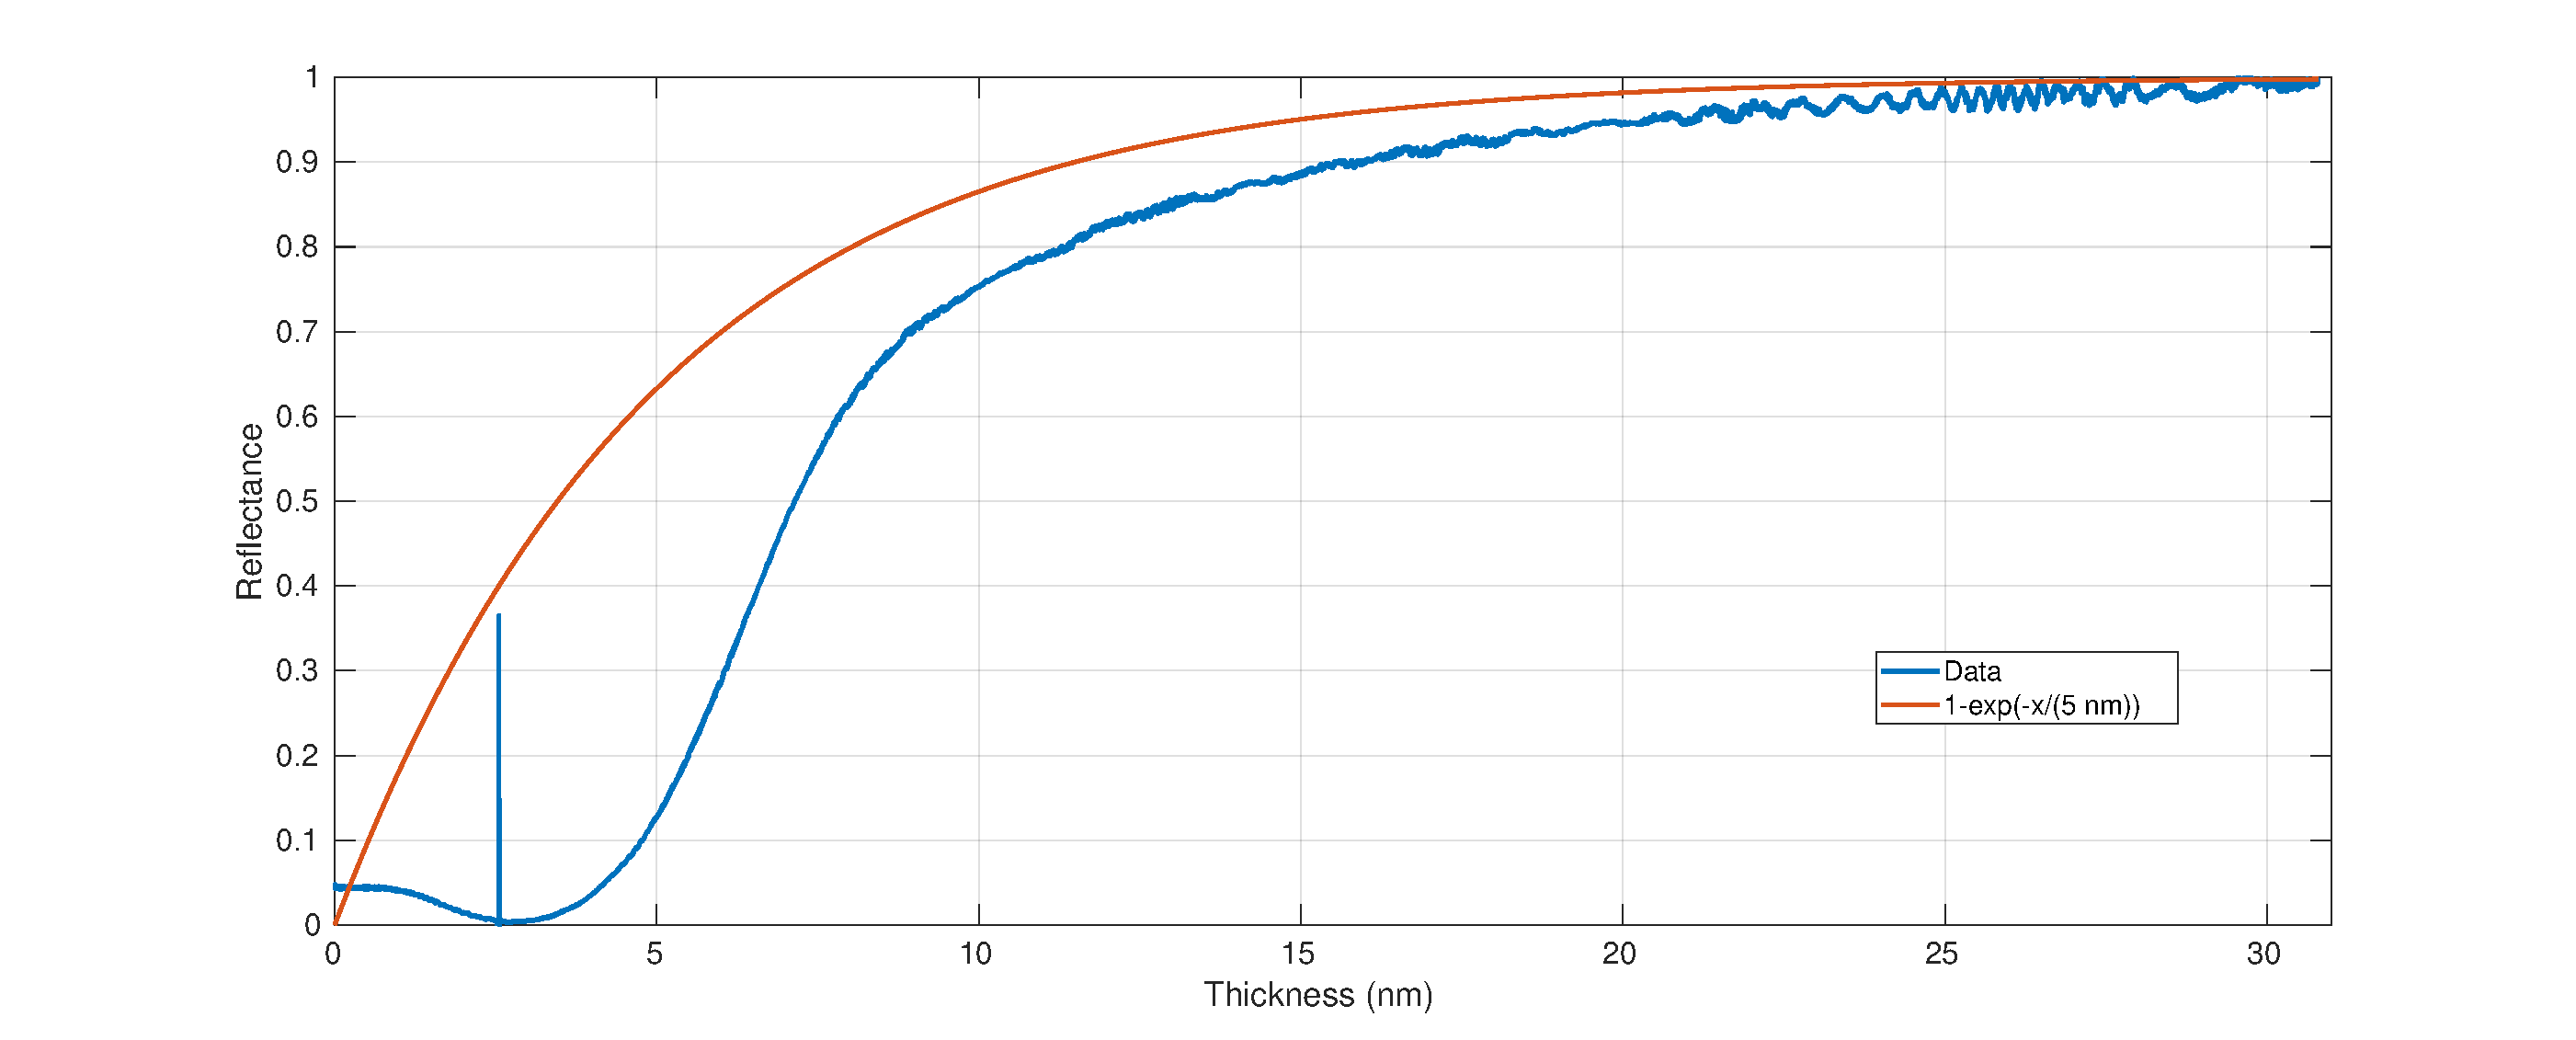
\includegraphics[width=\textwidth]{Gold_Coating_Fiber.pdf}
Above is an example run using this set-up where gold was added until the reflectance was close to 100\%. The curve does not follow the naive expectation from a skin depth picture which would predict an exponential decay to one with increased thickness. The true curve has a dip in reflectance with small thickness that is believed to be from a peak in the absorption due to the changing size of the gold islands as material is added. There is additionally some secondary interference which is believed to be caused by refections within the feedthrough.

\section{Example 50-50 Beamsplitter}
Below is an example of the creation of a roughly 50-50 beamsplitter. The sputtering was turned off at about 330 seconds which is then promptly followed by ringing of the secondary interference with a gradual rise. This rise is not representative of true increase of reflection as this fiber was measured after the fact to have a reflectance of 45\%.\\

\textbf{Settings:}

Initial Pressure: 3.4 $\mu$Torr

Final Thickness: 101\AA

Reflentance: 45\%

Time:  5 min 40 sec

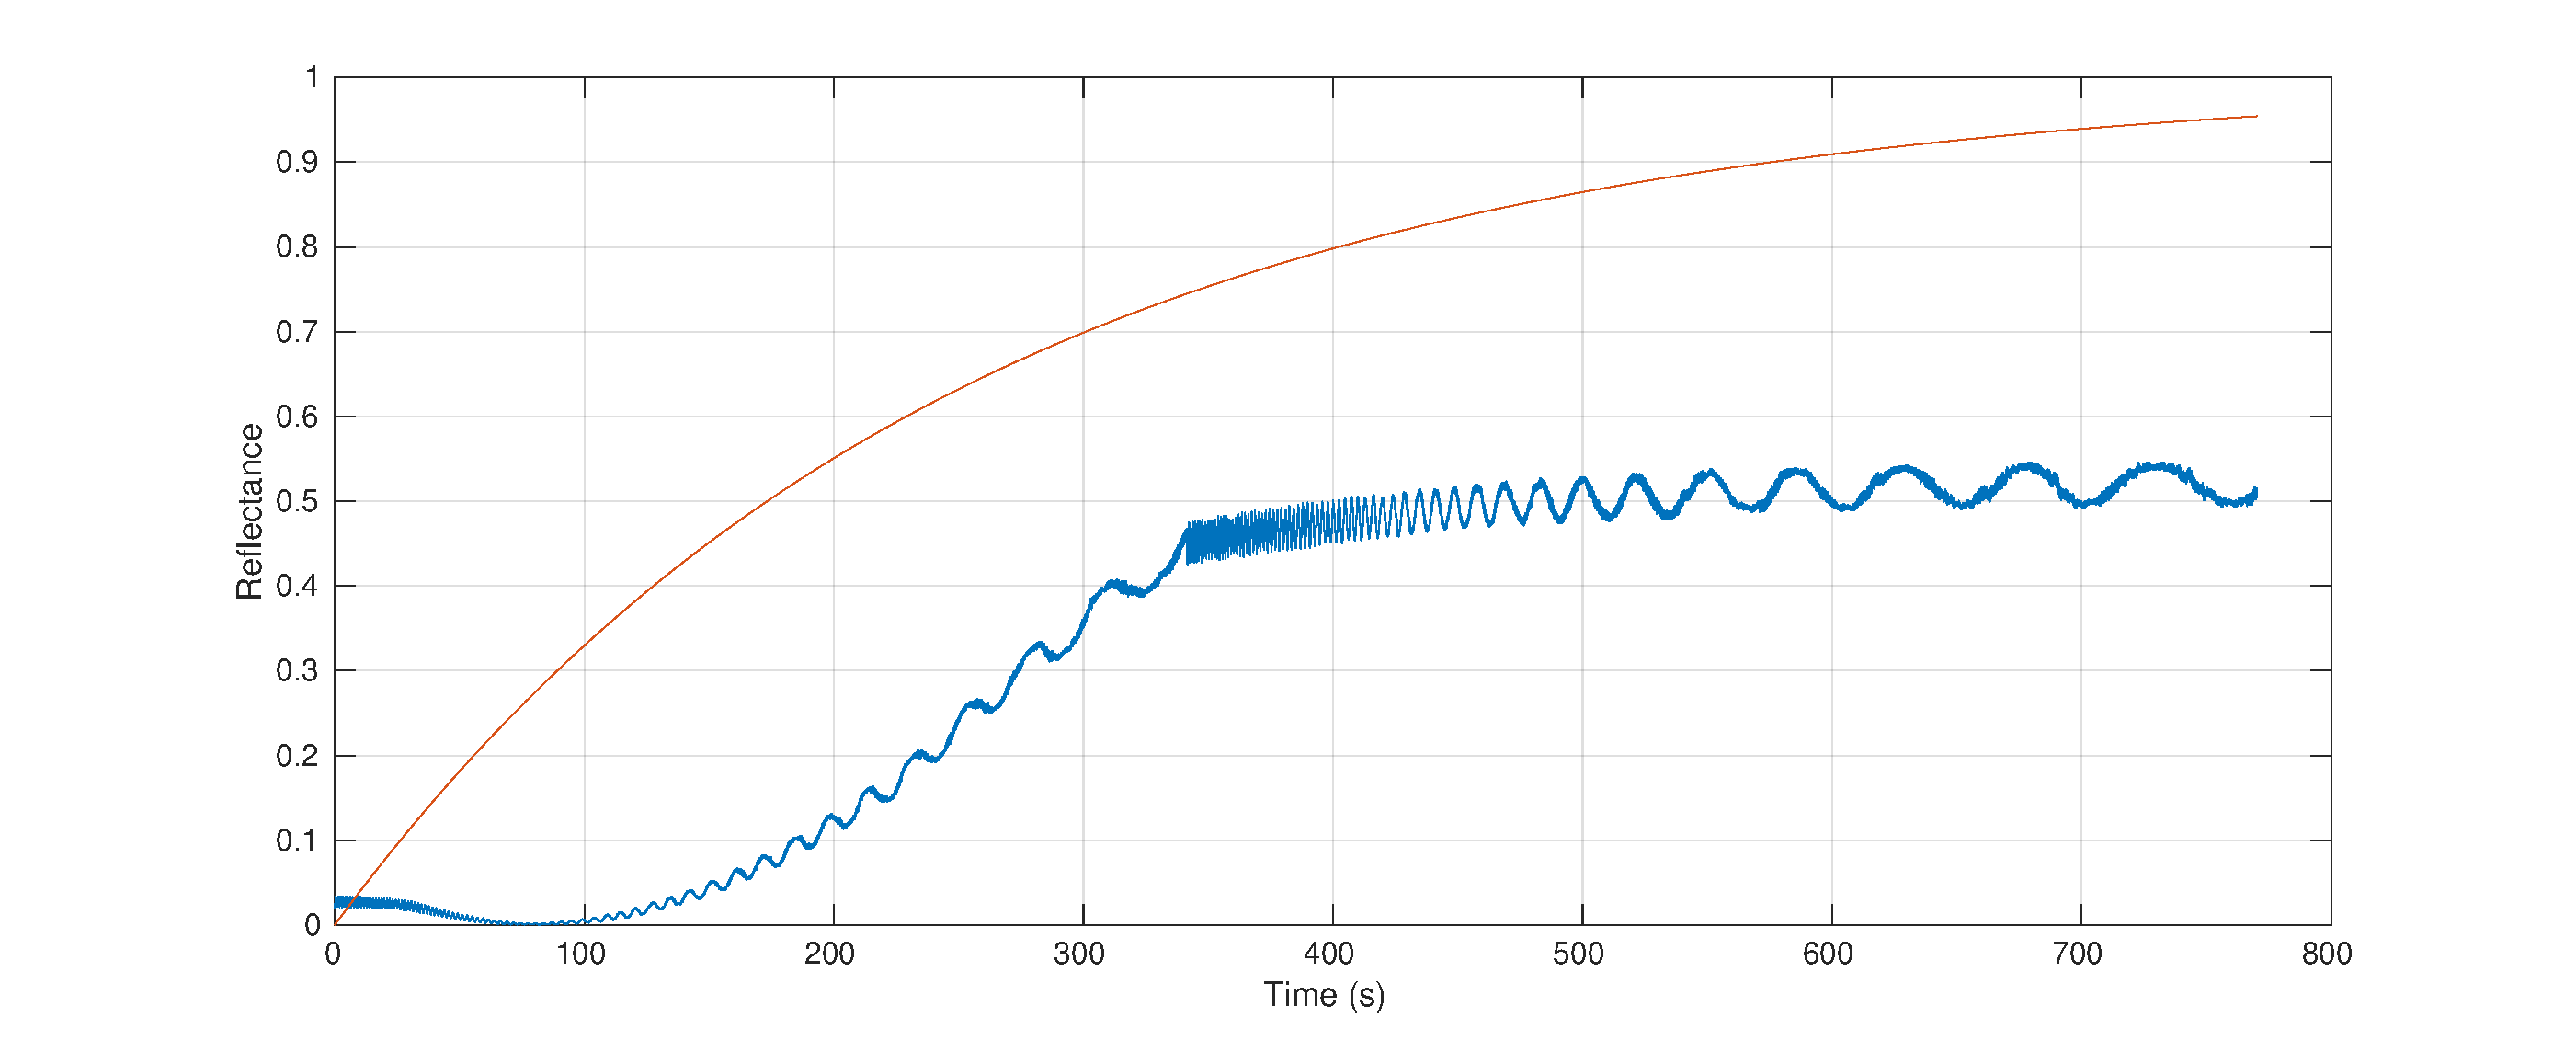
\includegraphics[width=\textwidth]{BS_Coating_Fiber_Time.pdf}

The following images show microscope images of this fiber at two separate zooms. It is apparent with these images that the gold is coating the ceramic ferule uniformly yet does not form a uniform layer on the fiber tip. This will increase the loss of the coating as some of the returning beam will be reflected into higher order fiber modes and thus attenuated as they propagate down the fiber.\\

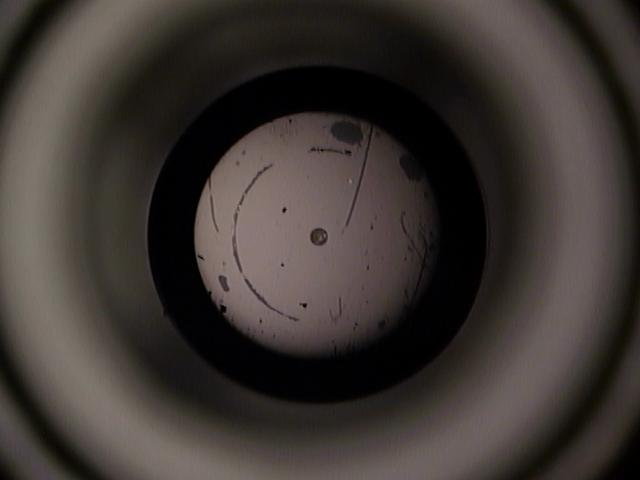
\includegraphics[width=0.5\textwidth]{GoldFiberTip.JPG}
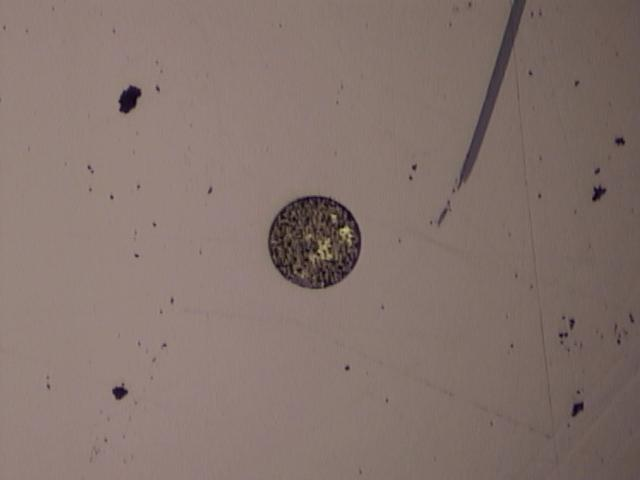
\includegraphics[width=0.5\textwidth]{GoldFiberTipZoom.JPG}
\section{References}
\begin{enumerate}
\item LIGO Vacuum Compatible Materials List (LIGO-E960050-v13)
\item Thorlabs Guide to Connectorization and Polishing Optical Fibers 
\end{enumerate}
\end{document}